\section{E2: Traffic with an obstacle}
\newcommand{\Ex}{E2}
The previous experiment demonstrates the superior performance of our proposed GM-PHD filter method, incorporating the dynamic detection probability and the modified pruning over the standard GM-PHD filter with the constant detection probability. Nevertheless, our method is initialy designed to excel in situations where obstacles obscure camera view. To assess its effectiveness in such scenarios, Experiment \textit{E2} is proposed.

\subsection{V3}
\newcommand{\Vs}{V3}
In video \textit{V3} a light pole is in camera's view, preventing the object detector to detect hidden objects. The video playback has been reduced to 10 fps.

\subsection{V3 - GM-PHD filter with the constant detection probability}
\newcommand{\Set}{S0}
The targets cannot persist beyond a certain number of time steps without being measured, resulting in their loss once they surpass an obstacle. To avert a permanent loss, a new spawning point is introduced immediately after the obstacle to revive the lost target. However, this approach comes with a drawback: the revived target starts afresh without retaining its previous history.

Parameter settings are embodied in Table \ref{tab:\Ex-\Vs-\Set}.

\begin{table}[!h]
    \centering
    \begin{tabular}{|c|c|c|c|c|c|}
        \hline
        $P_{D}$ & $P$ & $\sigma_{\upsilon}$ & $\sigma_{\epsilon}$ & $T_p$ & $T_{YOLO}$ \\ \noalign{\hrule height 1.5pt}
        0.9 & $diag(500,500,500,500)$ & 0.1 & 100 & 0.1 & 0.3\\
        \hline
    \end{tabular}
    \caption{The parameter settings for Experiment {\Ex-\Vs} with the constant detection probability.}
    \label{tab:\Ex-\Vs-\Set}
\end{table}

Figure \ref{fig:\Ex-\Vs-\Set} shows some highlights of the GM-PHD filter with the constant detection probability.

Here's a refined version of the passage for your thesis:

\begin{itemize}
    \item \textbf{\ref{fig:\Ex-\Vs-\Set:01}:} The sequence initiates at frame number 7, where the first car is initialized near the spawning point.
    \item \textbf{\ref{fig:\Ex-\Vs-\Set:02}:} The first car approaches an obstacle, coinciding with the arrival of the second car.
    \item \textbf{\ref{fig:\Ex-\Vs-\Set:03}:} The YOLO object detector fails to detect the obscured car, resulting in its removal from tracking.
    \item \textbf{\ref{fig:\Ex-\Vs-\Set:04}:} The previously lost target is rediscovered and initialized at the second spawning point. However, its tracking history remains incomplete, having not been tracked for five consecutive frames.
    \item \textbf{\ref{fig:\Ex-\Vs-\Set:05}:} The second car is obstructed from detection by the obstacle, leading to the loss of its tracking.
    \item \textbf{\ref{fig:\Ex-\Vs-\Set:06}:} The target is once again initialized at the second spawning point, coinciding with the approach of the third car.
    \item \textbf{\ref{fig:\Ex-\Vs-\Set:07}:} The final car, similarly concealed behind an obstacle, evades detection, resulting in the loss of its tracking.
    \item \textbf{\ref{fig:\Ex-\Vs-\Set:08}:} Despite the target being reinitialized, its tracking history remains unavailable for six consecutive frames. Additionally, the other two cars, distant and appearing to be in close proximity, are merged into a single target by the filter.
\end{itemize}




According to Graph \ref{gr:\Ex-\Vs-\Set}, the filter demonstrates commendable tracking performance for the targets. However, the graph also highlights a notable weakness of this approach, evident in the pronounced peaks indicating target loss.

With the introduction of the second spawn point facilitating target rebirth, the GM-PHD filter effectively maintains accurate tracking of all targets. Nonetheless, the inherent weakness of this strategy becomes apparent: when a target is reborn, it is treated as an entirely new target without any historical data.

\begin{figure}[H]
    \centering
    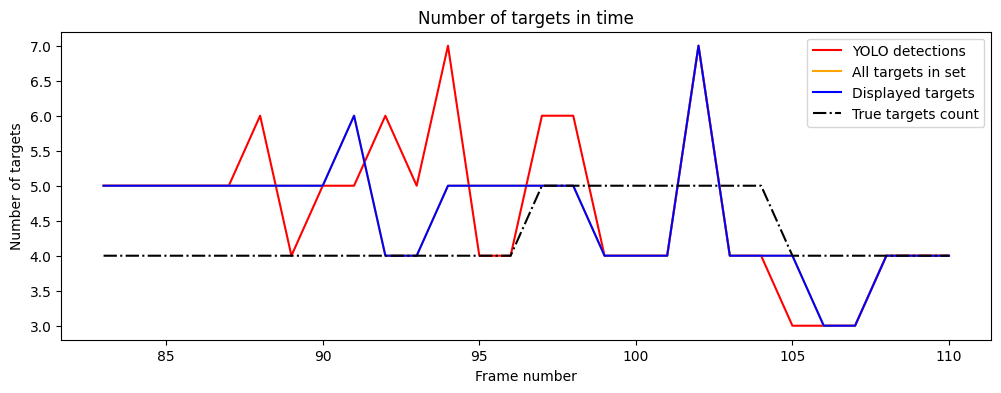
\includegraphics[width=\linewidth]{../../../experiments/\Ex/\Vs/noPd/staticPd_det}
    \caption{Development chart of the number of detected targets, targets in the filter's queue, displayed targets and true targets' count.}
    \label{gr:\Ex-\Vs-\Set}
\end{figure}

\begin{figure}[H]
    \centering
    \begin{subfigure}{0.23\textwidth}
        \centering
        \includegraphics[width=\linewidth]{../../../experiments/\Ex/\Vs/noPd/7}
        \caption{Frame number: 7.}
        \label{fig:\Ex-\Vs-\Set:01}
    \end{subfigure}
    \begin{subfigure}{0.23\textwidth}
        \centering
        \includegraphics[width=\linewidth]{../../../experiments/\Ex/\Vs/noPd/33}
        \caption{Frame number: 33.}
        \label{fig:\Ex-\Vs-\Set:02}
    \end{subfigure}
    \begin{subfigure}{0.23\textwidth}
        \centering
        \includegraphics[width=\linewidth]{../../../experiments/\Ex/\Vs/noPd/38}
        \caption{Frame number: 38.}
        \label{fig:\Ex-\Vs-\Set:03}
    \end{subfigure}
    \begin{subfigure}{0.23\textwidth}
        \centering
        \includegraphics[width=\linewidth]{../../../experiments/\Ex/\Vs/noPd/43}
        \caption{Frame number: 43.}
        \label{fig:\Ex-\Vs-\Set:04}
    \end{subfigure}
    \\
    \begin{subfigure}{0.23\textwidth}
        \centering
        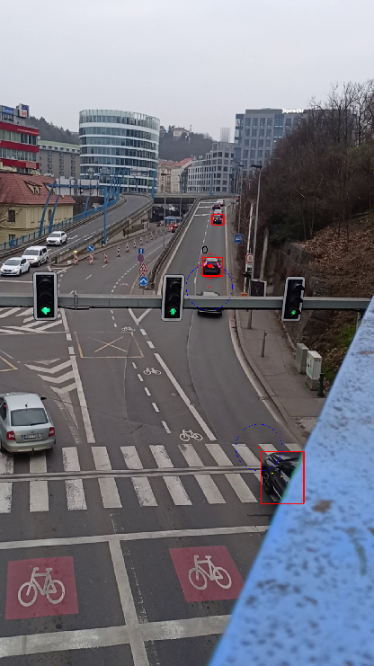
\includegraphics[width=\linewidth]{../../../experiments/\Ex/\Vs/noPd/55}
        \caption{Frame number: 55.}
        \label{fig:\Ex-\Vs-\Set:05}
    \end{subfigure}
    \begin{subfigure}{0.23\textwidth}
        \centering
        \includegraphics[width=\linewidth]{../../../experiments/\Ex/\Vs/noPd/60}
        \caption{Frame number: 60.}
        \label{fig:\Ex-\Vs-\Set:06}
    \end{subfigure}
    \begin{subfigure}{0.23\textwidth}
        \centering
        \includegraphics[width=\linewidth]{../../../experiments/\Ex/\Vs/noPd/85}
        \caption{Frame number: 85.}
        \label{fig:\Ex-\Vs-\Set:07}
    \end{subfigure}
    \begin{subfigure}{0.23\textwidth}
        \centering
        \includegraphics[width=\linewidth]{../../../experiments/\Ex/\Vs/noPd/92}
        \caption{Frame number: 92.}
        \label{fig:\Ex-\Vs-\Set:08}
    \end{subfigure}
    \caption{Image sequence of tracked objects using the GM-PHD filter with the constant detection probability.}
    \label{fig:\Ex-\Vs-\Set}
\end{figure}




\subsection{V3 -- GM-PHD with the dynamic detection probability}
Experiments on the video \textit{V3} using the GM-PHD filter with the dynamic detection probability and settings \textit{S1, S2, S3} are
demonstrated in following sections.
\subsubsection{S1 -- YOLO + YOLO}
\renewcommand{\Set}{S1}
This experiment uses settings \textit{S1}, where the YOLO model provides with both object detection bboxes and
segmentation masks.
The parameter settings are shown in Table \ref{tab:\Ex-\Vs-\Set}.
\begin{table}[H]
    \centering
    \begin{tabular}{|c|c|c|c|c|c|c|c|c|}
        \hline
        $P_{D,k}(x)$ & $P$ & $\sigma_{\upsilon}$ & $\sigma_{\epsilon}$ & $T_H$ & $T_d$ & $T_p$ & $T_l$ & $T_{YOLO}$ \\ \noalign{\hrule
        height 1.5pt}
        0.3 & $diag(500,500,500,500)$ & 0.1 & 100 & 2 & 3 & 0.1 & 0.0001 & 0.3\\
        \hline
    \end{tabular}
    \caption{The parameter settings for Experiment {\Ex-\Vs-\Set} with the dynamic detection probability.}
    \label{tab:\Ex-\Vs-\Set}
\end{table}

Figure \ref{fig:\Ex-\Vs-\Set} shows the performance of the GM-PHD filter with the dynamic detection probability with settings \textit{S1}.
\begin{itemize}
    \item \textbf{\ref{fig:\Ex-\Vs-\Set:01}:} Tracking commences at frame number 7, with the first target approaching the spawning point.
    \item \textbf{\ref{fig:\Ex-\Vs-\Set:02}:} The first car reaches the light pole, coinciding with the appearance of the second car in the scene.
    \item \textbf{\ref{fig:\Ex-\Vs-\Set:03}:} This marks the last detection of YOLO of the first car before encountering the obstacle.
    \item \textbf{\ref{fig:\Ex-\Vs-\Set:04}:} Despite the first car not being detected for 5 frames, it successfully persists without the need for the second spawning point.
    \item \textbf{\ref{fig:\Ex-\Vs-\Set:05}:} This frame illustrates an example of a \textit{hidden} target state, where the second car is annotated with number 1, indicating it is considered as hidden.
    \item \textbf{\ref{fig:\Ex-\Vs-\Set:06}:} The second car surpasses the obstacle and continues along its trajectory, demonstrating its ability to survive for 6 consecutive time steps.
    \item \textbf{\ref{fig:\Ex-\Vs-\Set:07}:} With the two cars appearing close to each other, additional measurements emerge within the validation region of the targets. Despite the third car not being detected behind the light pole, it is still successfully tracked.
    \item \textbf{\ref{fig:\Ex-\Vs-\Set:08}:} The targets of the first two cars are merged together due to their long distance from the camera and the presence of static motion and observation noises. Additionally, the third target also survives the period of misdetection.
\end{itemize}

The displayed targets line in Graph \ref{gr:\Ex-\Vs-\Set} is almost the same as in previous experiment. However, the orange line shows that the filter is still informed about all potential targets. As seen in \ref{fig:\Ex-\Vs-\Set} the hidden targets are not lost, their weights are just too small to be displayed.

The performance of the GM-PHD filter with the dynamic detection probability might seem to be very similar to the constant detection probability at first glance. But the targets are not removed when hidden. Moreover, the targets' track history is not lost.

\begin{figure}[H]
    \centering
    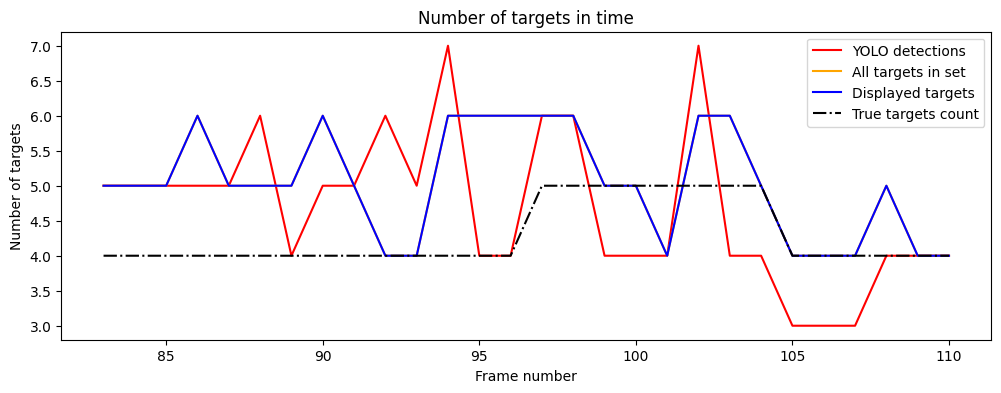
\includegraphics[width=\linewidth]{../../../experiments/\Ex/\Vs/YOLO/yolo_det}
    \caption{Development chart of the number of detected targets, targets in the filter's queue, displayed targets and true targets' count.}
    \label{gr:\Ex-\Vs-\Set}
\end{figure}

\begin{figure}[H]
    \centering
    \begin{subfigure}{0.23\textwidth}
        \centering
        \includegraphics[width=\linewidth]{../../../experiments/\Ex/\Vs/YOLO/7}
        \caption{Frame number: 7.}
        \label{fig:\Ex-\Vs-\Set:01}
    \end{subfigure}
    \begin{subfigure}{0.23\textwidth}
        \centering
        \includegraphics[width=\linewidth]{../../../experiments/\Ex/\Vs/YOLO/33}
        \caption{Frame number: 33.}
        \label{fig:\Ex-\Vs-\Set:02}
    \end{subfigure}
    \begin{subfigure}{0.23\textwidth}
        \centering
        \includegraphics[width=\linewidth]{../../../experiments/\Ex/\Vs/YOLO/38}
        \caption{Frame number: 38.}
        \label{fig:\Ex-\Vs-\Set:03}
    \end{subfigure}
    \begin{subfigure}{0.23\textwidth}
        \centering
        \includegraphics[width=\linewidth]{../../../experiments/\Ex/\Vs/YOLO/43}
        \caption{Frame number: 43.}
        \label{fig:\Ex-\Vs-\Set:04}
    \end{subfigure}
    \\
    \begin{subfigure}{0.23\textwidth}
        \centering
        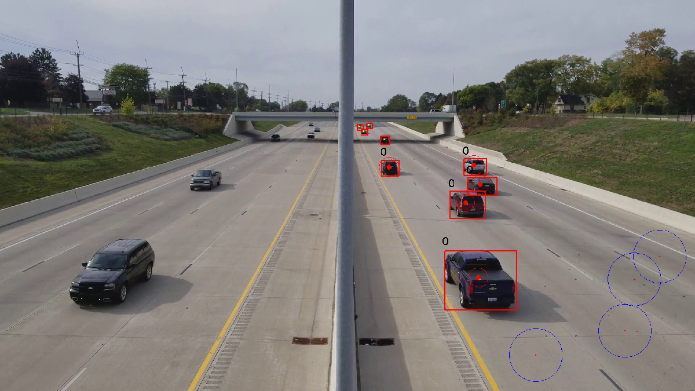
\includegraphics[width=\linewidth]{../../../experiments/\Ex/\Vs/YOLO/58}
        \caption{Frame number: 58.}
        \label{fig:\Ex-\Vs-\Set:05}
    \end{subfigure}
    \begin{subfigure}{0.23\textwidth}
        \centering
        \includegraphics[width=\linewidth]{../../../experiments/\Ex/\Vs/YOLO/60}
        \caption{Frame number: 60.}
        \label{fig:\Ex-\Vs-\Set:06}
    \end{subfigure}
    \begin{subfigure}{0.23\textwidth}
        \centering
        \includegraphics[width=\linewidth]{../../../experiments/\Ex/\Vs/YOLO/85}
        \caption{Frame number: 85.}
        \label{fig:\Ex-\Vs-\Set:07}
    \end{subfigure}
    \begin{subfigure}{0.23\textwidth}
        \centering
        \includegraphics[width=\linewidth]{../../../experiments/\Ex/\Vs/YOLO/92}
        \caption{Frame number: 92.}
        \label{fig:\Ex-\Vs-\Set:08}
    \end{subfigure}
    \caption{Image sequence of tracked objects using the GM-PHD filter with the dynamic detection probability and YOLO only.}
    \label{fig:\Ex-\Vs-\Set}
\end{figure}




\subsubsection{S2 -- YOLO + SAM}
\renewcommand{\Set}{S2}
The next settings employs settings \textit{S2} with the YOLO object detector and the SAM
segmentation model on the video \textit{V3}.

All parameters are encompassed within Table \ref{tab:\Ex-\Vs-\Set}.
\begin{table}[H]
    \centering
    \begin{tabular}{|c|c|c|c|c|c|c|c|c|}
        \hline
        $P_{D,k}(x)$ & $P$ & $\sigma_{\upsilon}$ & $\sigma_{\epsilon}$ & $T_H$ & $T_d$ & $T_p$ & $T_l$ & $T_{YOLO}$ \\ \noalign{\hrule
        height 1.5pt}
        0.3 & $diag(500,500,500,500)$ & 0.1 & 100 & 2 & 3 & 0.1 & 0.0001 & 0.3\\
        \hline
    \end{tabular}
    \caption{The parameter settings for Experiment {\Ex-\Vs-\Set} with the dynamic detection probability.}
    \label{tab:\Ex-\Vs-\Set}
\end{table}


The scenario in \ref{fig:\Ex-\Vs-\Set} is almost exactly the same as in experiment with settings \textit{S1}. All targets are tracked properly and none of them are lost.


Graph \ref{gr:\Ex-\Vs-\Set} vividly illustrates the discernible disparity between settings \textit{S1} and \textit{S2}. The blue line deviates less from the true count, and notably, in scenarios where targets are obscured, the number of targets in the filter's queue (orange line) mirrors the true count line. It is only from frame number 80 onwards that the orange line exhibits some errors, attributed to the targets appearing in the same neighborhood.


Once again, settings \textit{S2} demonstrate a slightly superior performance compared to settings \textit{S1}. The substantial improvement is distinctly evident in Graph \ref{gr:\Ex-\Vs-\Set}.

\begin{figure}[H]
    \centering
    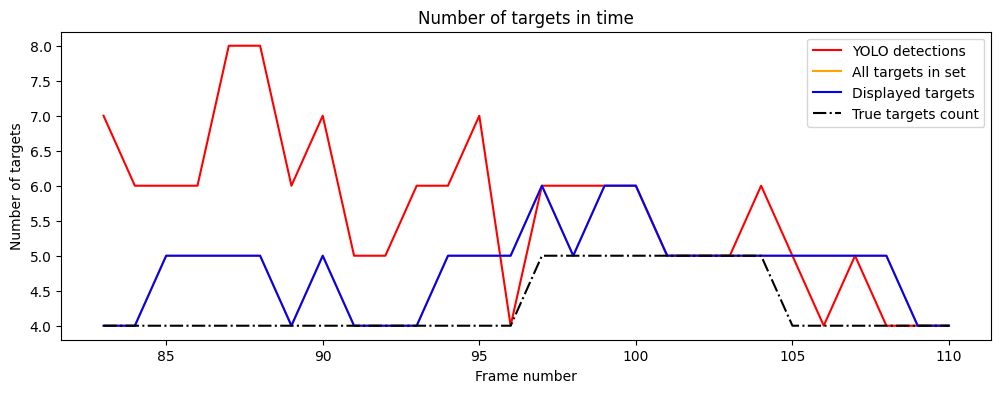
\includegraphics[width=\linewidth]{../../../experiments/\Ex/\Vs/SAM/sam_det}
    \caption{Development chart of the number of detected targets, targets in the filter's queue, displayed targets and true targets' count.}
    \label{gr:\Ex-\Vs-\Set}
\end{figure}

\begin{figure}[H]
    \centering
    \begin{subfigure}{0.23\textwidth}
        \centering
        \includegraphics[width=\linewidth]{../../../experiments/\Ex/\Vs/SAM/7}
        \caption{Frame number: 7}
        \label{fig:\Ex-\Vs-\Set:01}
    \end{subfigure}
    \begin{subfigure}{0.23\textwidth}
        \centering
        \includegraphics[width=\linewidth]{../../../experiments/\Ex/\Vs/SAM/33}
        \caption{Frame number: 33.}
        \label{fig:\Ex-\Vs-\Set:02}
    \end{subfigure}
    \begin{subfigure}{0.23\textwidth}
        \centering
        \includegraphics[width=\linewidth]{../../../experiments/\Ex/\Vs/SAM/38}
        \caption{Frame number: 38.}
        \label{fig:\Ex-\Vs-\Set:03}
    \end{subfigure}
    \begin{subfigure}{0.23\textwidth}
        \centering
        \includegraphics[width=\linewidth]{../../../experiments/\Ex/\Vs/SAM/43}
        \caption{Frame number: 43.}
        \label{fig:\Ex-\Vs-\Set:04}
    \end{subfigure}
    \\
    \begin{subfigure}{0.23\textwidth}
        \centering
        \includegraphics[width=\linewidth]{../../../experiments/\Ex/\Vs/SAM/57}
        \caption{Frame number: 57.}
        \label{fig:\Ex-\Vs-\Set:05}
    \end{subfigure}
    \begin{subfigure}{0.23\textwidth}
        \centering
        \includegraphics[width=\linewidth]{../../../experiments/\Ex/\Vs/SAM/60}
        \caption{Frame number: 60.}
        \label{fig:\Ex-\Vs-\Set:06}
    \end{subfigure}
    \begin{subfigure}{0.23\textwidth}
        \centering
        \includegraphics[width=\linewidth]{../../../experiments/\Ex/\Vs/SAM/85}
        \caption{Frame number: 85.}
        \label{fig:\Ex-\Vs-\Set:07}
    \end{subfigure}
    \begin{subfigure}{0.23\textwidth}
        \centering
        \includegraphics[width=\linewidth]{../../../experiments/\Ex/\Vs/SAM/92}
        \caption{Frame number: 92.}
        \label{fig:\Ex-\Vs-\Set:08}
    \end{subfigure}
    \caption{Image sequence of tracked objects using the GM-PHD filter with the dynamic detection probability, the YOLO object detector and the SAM image segmentation model.}
    \label{fig:\Ex-\Vs-\Set}
\end{figure}


\subsubsection{S3 -- Grounded SAM}
\renewcommand{\Set}{S3}
The combination of Grounding DINO and SAM is also evaluated on the video \textit{V3}. The parameters utilized are outlined in Table \ref{tab:\Ex-\Vs-\Set}.
\begin{table}[H]
    \centering
    \begin{tabular}{|c|c|c|c|c|c|c|c|c|c|}
        \hline
        $P_{D,k}(x)$ & $P$ & $\sigma_{\upsilon}$ & $\sigma_{\epsilon}$ & $T_H$ & $T_d$ & $T_p$ & $T_l$ & $T_{text}$ & $T_{bbox}$\\ \noalign{\hrule
        height 1.5pt}
        0.3 & $diag(500,500,500,500)$ & 0.1 & 80 & 2 & 3 & 0.1 & 0.01 & 0.3 & 0.3\\
        \hline
    \end{tabular}
    \caption{The parameter settings for Experiment {\Ex-\Vs-\Set} with the dynamic detection probability.}
    \label{tab:\Ex-\Vs-\Set}
\end{table}

As seen in Figures \ref{fig:\Ex-\Vs-\Set:03}, \ref{fig:\Ex-\Vs-\Set:05} and \ref{fig:\Ex-\Vs-\Set:07}, Grounding DINO is able to detect the hidden objects behind the light pole, thus the advantage of the dynamic detection probability is not apparent. All targets are tracked precisely and no misdetection is present.

Until frame number 85, both the number of displayed targets (blue line) and the number of targets in the filter's queue (orange line) precisely mirror the true number of targets line. This alignment is attributed to the enhanced performance of the object detector, which successfully detects semi-hidden targets. However, the fluctuations in the number of targets observed after frame 85 are a result of targets being in close proximity to each other.

\begin{figure}[H]
    \centering
    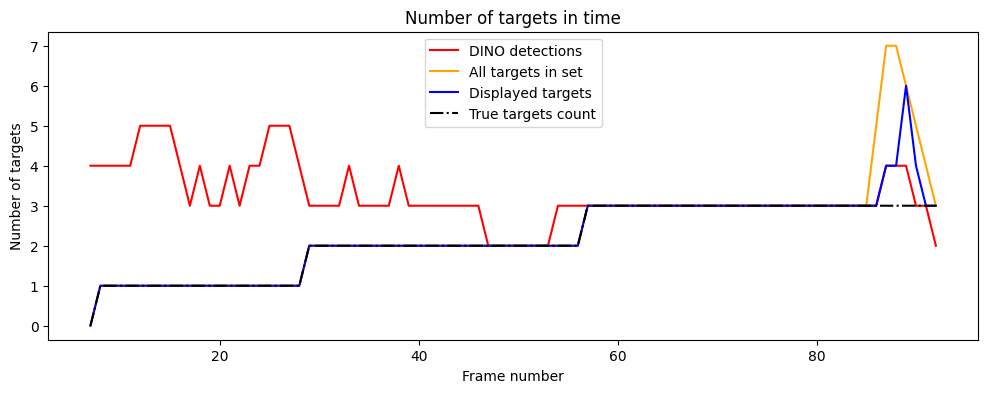
\includegraphics[width=\linewidth]{../../../experiments/\Ex/\Vs/DINO/dino_det}
    \caption{Development chart of the number of detected targets, targets in the filter's queue, displayed targets and true targets' count.}
    \label{gr:\Ex-\Vs-\Set}
\end{figure}

\begin{figure}[H]
    \centering
    \begin{subfigure}{0.23\textwidth}
        \centering
        \includegraphics[width=\linewidth]{../../../experiments/\Ex/\Vs/DINO/7}
        \caption{Frame number: 7.}
        \label{fig:\Ex-\Vs-\Set:01}
    \end{subfigure}
    \begin{subfigure}{0.23\textwidth}
        \centering
        \includegraphics[width=\linewidth]{../../../experiments/\Ex/\Vs/DINO/33}
        \caption{Frame number: 33.}
        \label{fig:\Ex-\Vs-\Set:02}
    \end{subfigure}
    \begin{subfigure}{0.23\textwidth}
        \centering
        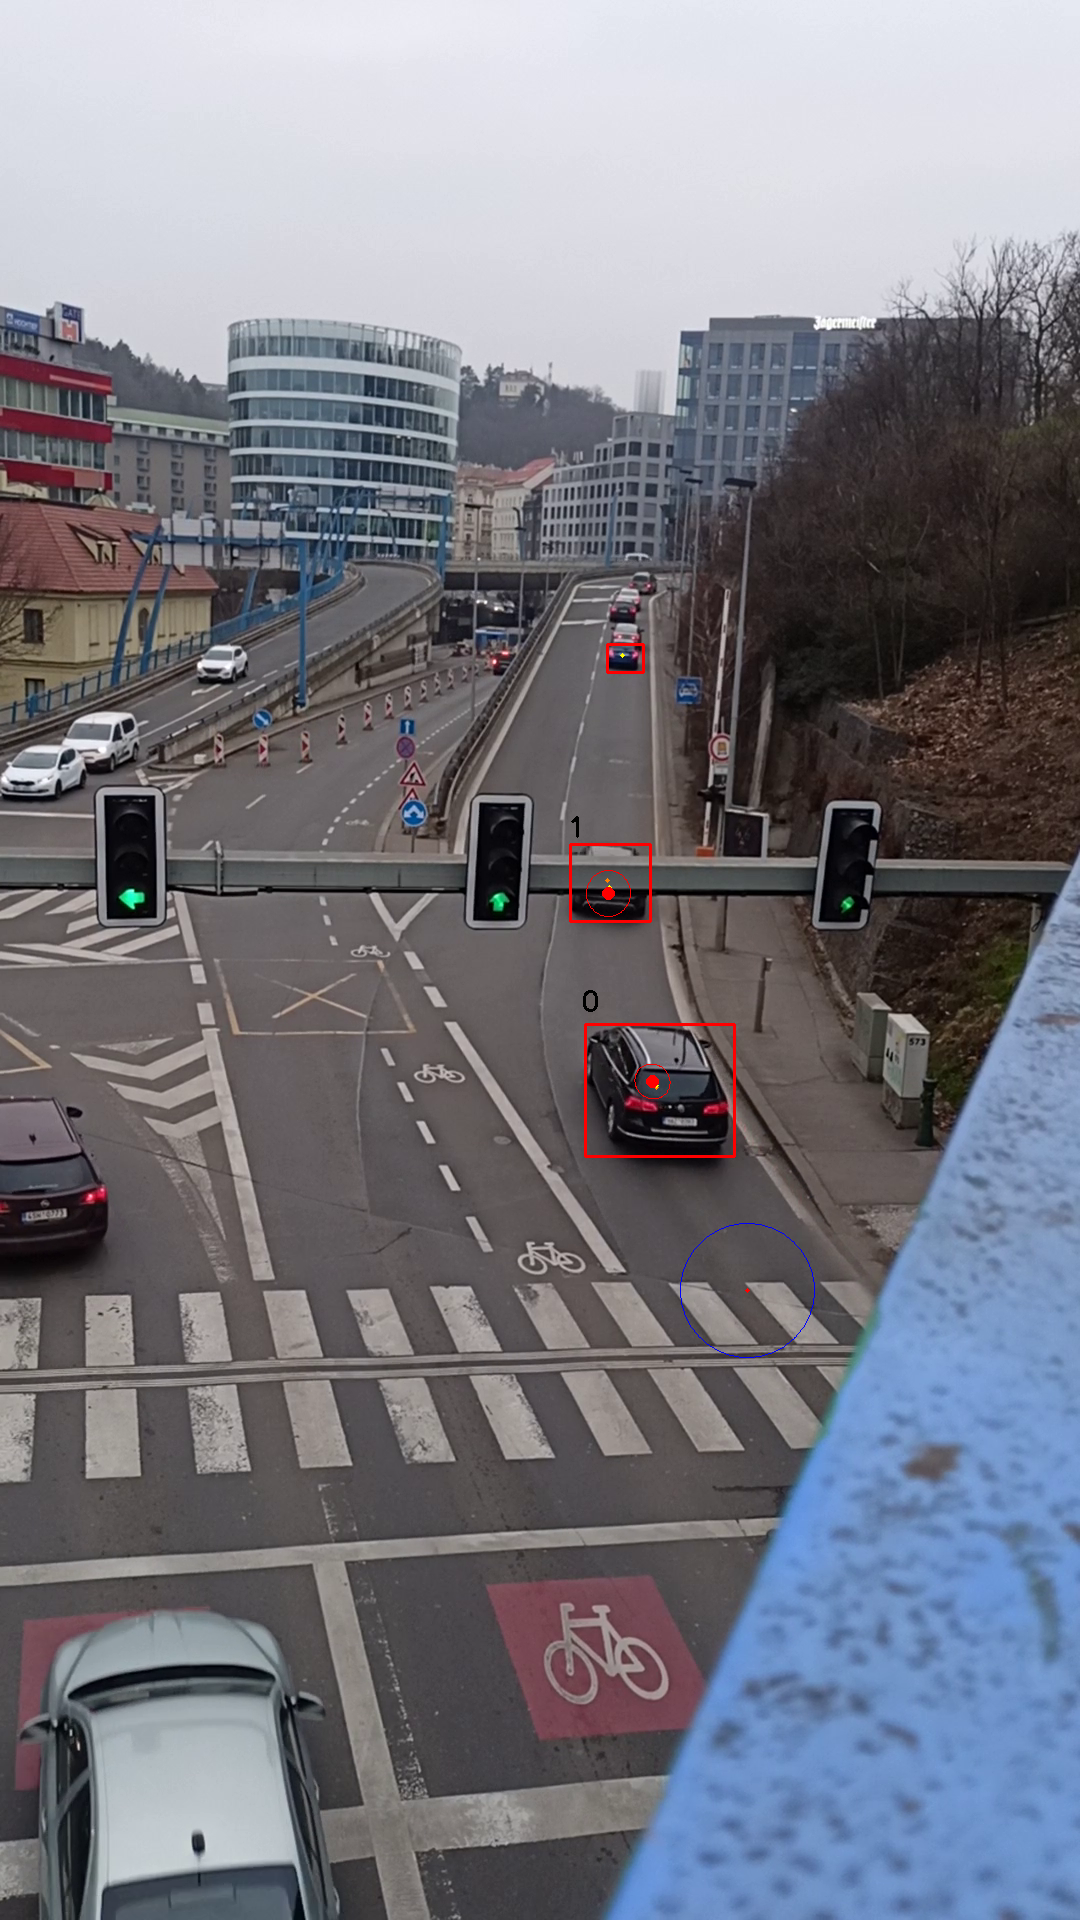
\includegraphics[width=\linewidth]{../../../experiments/\Ex/\Vs/DINO/39}
        \caption{Frame number: 39.}
        \label{fig:\Ex-\Vs-\Set:03}
    \end{subfigure}
    \begin{subfigure}{0.23\textwidth}
        \centering
        \includegraphics[width=\linewidth]{../../../experiments/\Ex/\Vs/DINO/43}
        \caption{Frame number: 43.}
        \label{fig:\Ex-\Vs-\Set:04}
    \end{subfigure}
    \\
    \begin{subfigure}{0.23\textwidth}
        \centering
        \includegraphics[width=\linewidth]{../../../experiments/\Ex/\Vs/DINO/57}
        \caption{Frame number: 57.}
        \label{fig:\Ex-\Vs-\Set:05}
    \end{subfigure}
    \begin{subfigure}{0.23\textwidth}
        \centering
        \includegraphics[width=\linewidth]{../../../experiments/\Ex/\Vs/DINO/60}
        \caption{Frame number: 60.}
        \label{fig:\Ex-\Vs-\Set:06}
    \end{subfigure}
    \begin{subfigure}{0.23\textwidth}
        \centering
        \includegraphics[width=\linewidth]{../../../experiments/\Ex/\Vs/DINO/85}
        \caption{Frame number: 85.}
        \label{fig:\Ex-\Vs-\Set:07}
    \end{subfigure}
    \begin{subfigure}{0.23\textwidth}
        \centering
        \includegraphics[width=\linewidth]{../../../experiments/\Ex/\Vs/DINO/92}
        \caption{Frame number: 92.}
        \label{fig:\Ex-\Vs-\Set:08}
    \end{subfigure}
    \caption{Image sequence of tracked objects using the GM-PHD filter with the dynamic detection probability, the DINO object detector and the SAM image segmentation model.}
    \label{fig:\Ex-\Vs-\Set}
\end{figure}




}